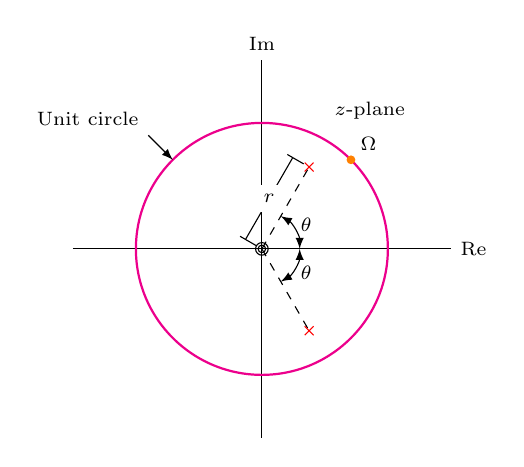
\begin{tikzpicture}[scale=0.8]
    \def\pole{++(135:0.1) -- ++(-45:0.2) ++(135:0.1) -- ++(45:0.1) -- ++(-135:0.2) +(45:0.1)}
    \def\zero{circle (0.1)}
    	\begin{scope}
     		%\path [pattern color=pink, pattern=north east lines] (-3, -3)  rectangle (3, 3);
     		%\draw [dashed, pattern color=pink, pattern=north east lines] (0,0) circle (2);
     		%\draw [dashed, fill=white] (0,0) circle (1/3);     		
	\end{scope}

    \draw (-3, 0) -- (3,0) node[anchor=west] {\scriptsize $\mathrm{Re}$};
    \draw (0, -3) -- (0,3) node[anchor=south] {\scriptsize $\mathrm{Im}$};
    %\pause
    \draw[thick, magenta] (0,0) circle (2);
    \draw [latex-] (0,0) ++(135:2) -- ++(135:0.55) node [anchor=south east] {\scriptsize Unit circle};

    \node at (1, 2.2) [anchor=west] {\scriptsize $z$-plane};
    %\draw (2, 0) node[anchor=north west] {$1$} \pole;
    
    
    \draw[dashed] (0,0) -- ++(60:1.5);
    \draw[red] (60:1.5) \pole;
   \draw[dashed] (0,0) -- ++(-60:1.5);
   \draw[red] (-60:1.5) \pole;    
    %\draw (1/3, 0) node[anchor=north ] {$\frac{1}{3}$} \pole;
	\draw    (0,0) \zero;
	\draw (0,0) circle (0.06);
	
	\draw[orange, fill] (45:2) circle (0.06) node[anchor=south west, text=black] {\scriptsize $\Omega$};
	\draw[latex-latex] (0.6, 0) arc (0:60:0.6);
	\draw[latex-latex] (0.6, 0) arc (0:-60:0.6);	
	\node at (40:0.6) [anchor= west] {\scriptsize $\theta$};
	\node at (-40:0.6) [anchor= west] {\scriptsize $\theta$};

	\draw[thin] (0,0)++(150:0.1) -- ++(150:0.3) ++(-30:0.1) -- node[fill=white] {\scriptsize $r$}++(60:1.5) ++(150:0.1) -- ++(-30:0.3);
\end{tikzpicture} 